\documentclass[12pt,letterpaper]{article}
\usepackage[utf8]{inputenc}
\usepackage{amsmath}
\usepackage{amsfonts}
\usepackage{amssymb}
\usepackage{amsthm}
\usepackage{graphicx}

\usepackage{hyperref}
\hypersetup{
    colorlinks=true,
    linkcolor=blue,
    filecolor=magenta,      
    urlcolor=cyan,
}
\urlstyle{same}

\usepackage{tabularx}
\usepackage[left=2cm,right=2cm,top=2cm,bottom=2cm]{geometry}
\usepackage{fancyhdr}
\usepackage{multicol}
\usepackage{multirow,array}
\usepackage{newtxtext,newtxmath}
\usepackage{relsize}
\usepackage{lastpage}
\usepackage{enumitem}
\usepackage{pdfpages}
\usepackage{adjustbox}
\newcolumntype{Y}{>{\centering\arraybackslash}X}
	\setenumerate[1]{label={\bf Q\theenumi: ~}}
	\setenumerate[2]{label={\bf \theenumii: ~}}
\pagestyle{fancy}
\fancyhf{}
\lhead{BHCC Mat-181}
\rhead{\textsc{Standard Normal Distribution}}
\rfoot{Page \thepage ~of \pageref*{LastPage}}

\newcommand{\N}[2]{\mathcal{N}\Big(#1,~ #2\Big)}


\begin{document}
The random variable $Z$ is normally distributed such that $\mu=0$ and $\sigma=1$. 
$$Z\sim \N{0}{1} $$
To determine the probability that $Z$ is less than $z_0$ (this is also the percentile of $z_0$), we find the area under the curve from $-\infty$ to $z_0$.
$$P(Z<z_0) ~=~ \text{Left area up to }z_0 $$
\begin{center}
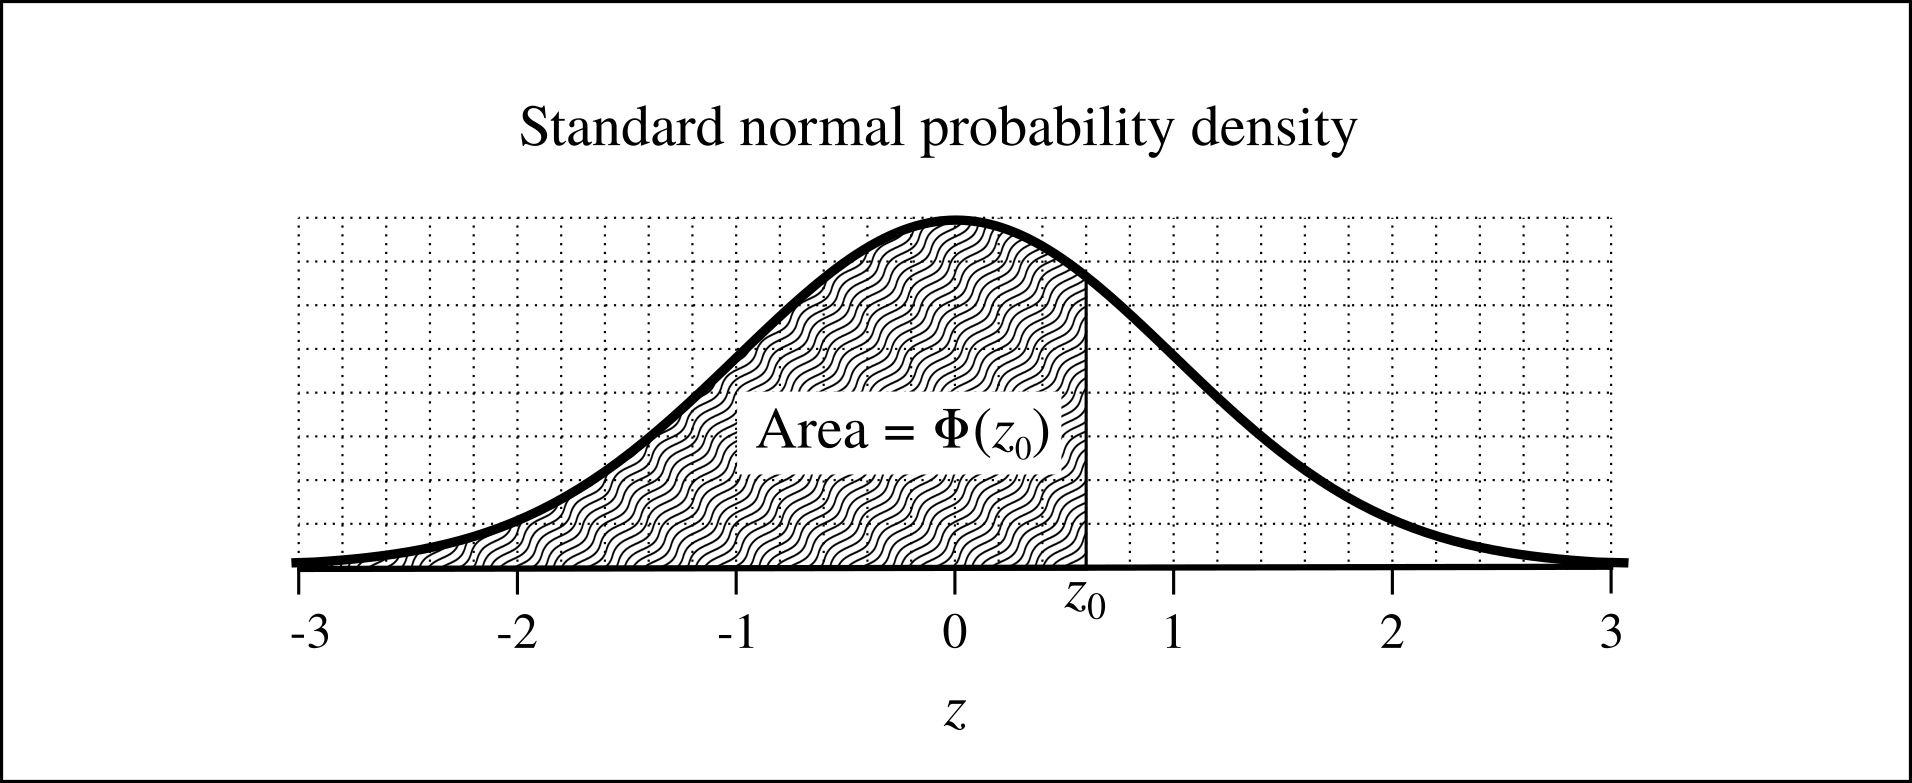
\includegraphics[scale=.85]{snpdarea2.png}
\end{center}
We use $\Phi$, an upper-case ``Phi'', to represent a left area of the standard normal density. We know $\Phi$ depends on $z_0$, so we use function notation. Also, we call this function the {\bf standard normal cumulative function}.
$$\Phi(z_0) \equiv P(Z<z_0) $$
If we repeat the process of finding the areas from $-\infty$ to any $z$, we get the cumulative function. 
\begin{center}
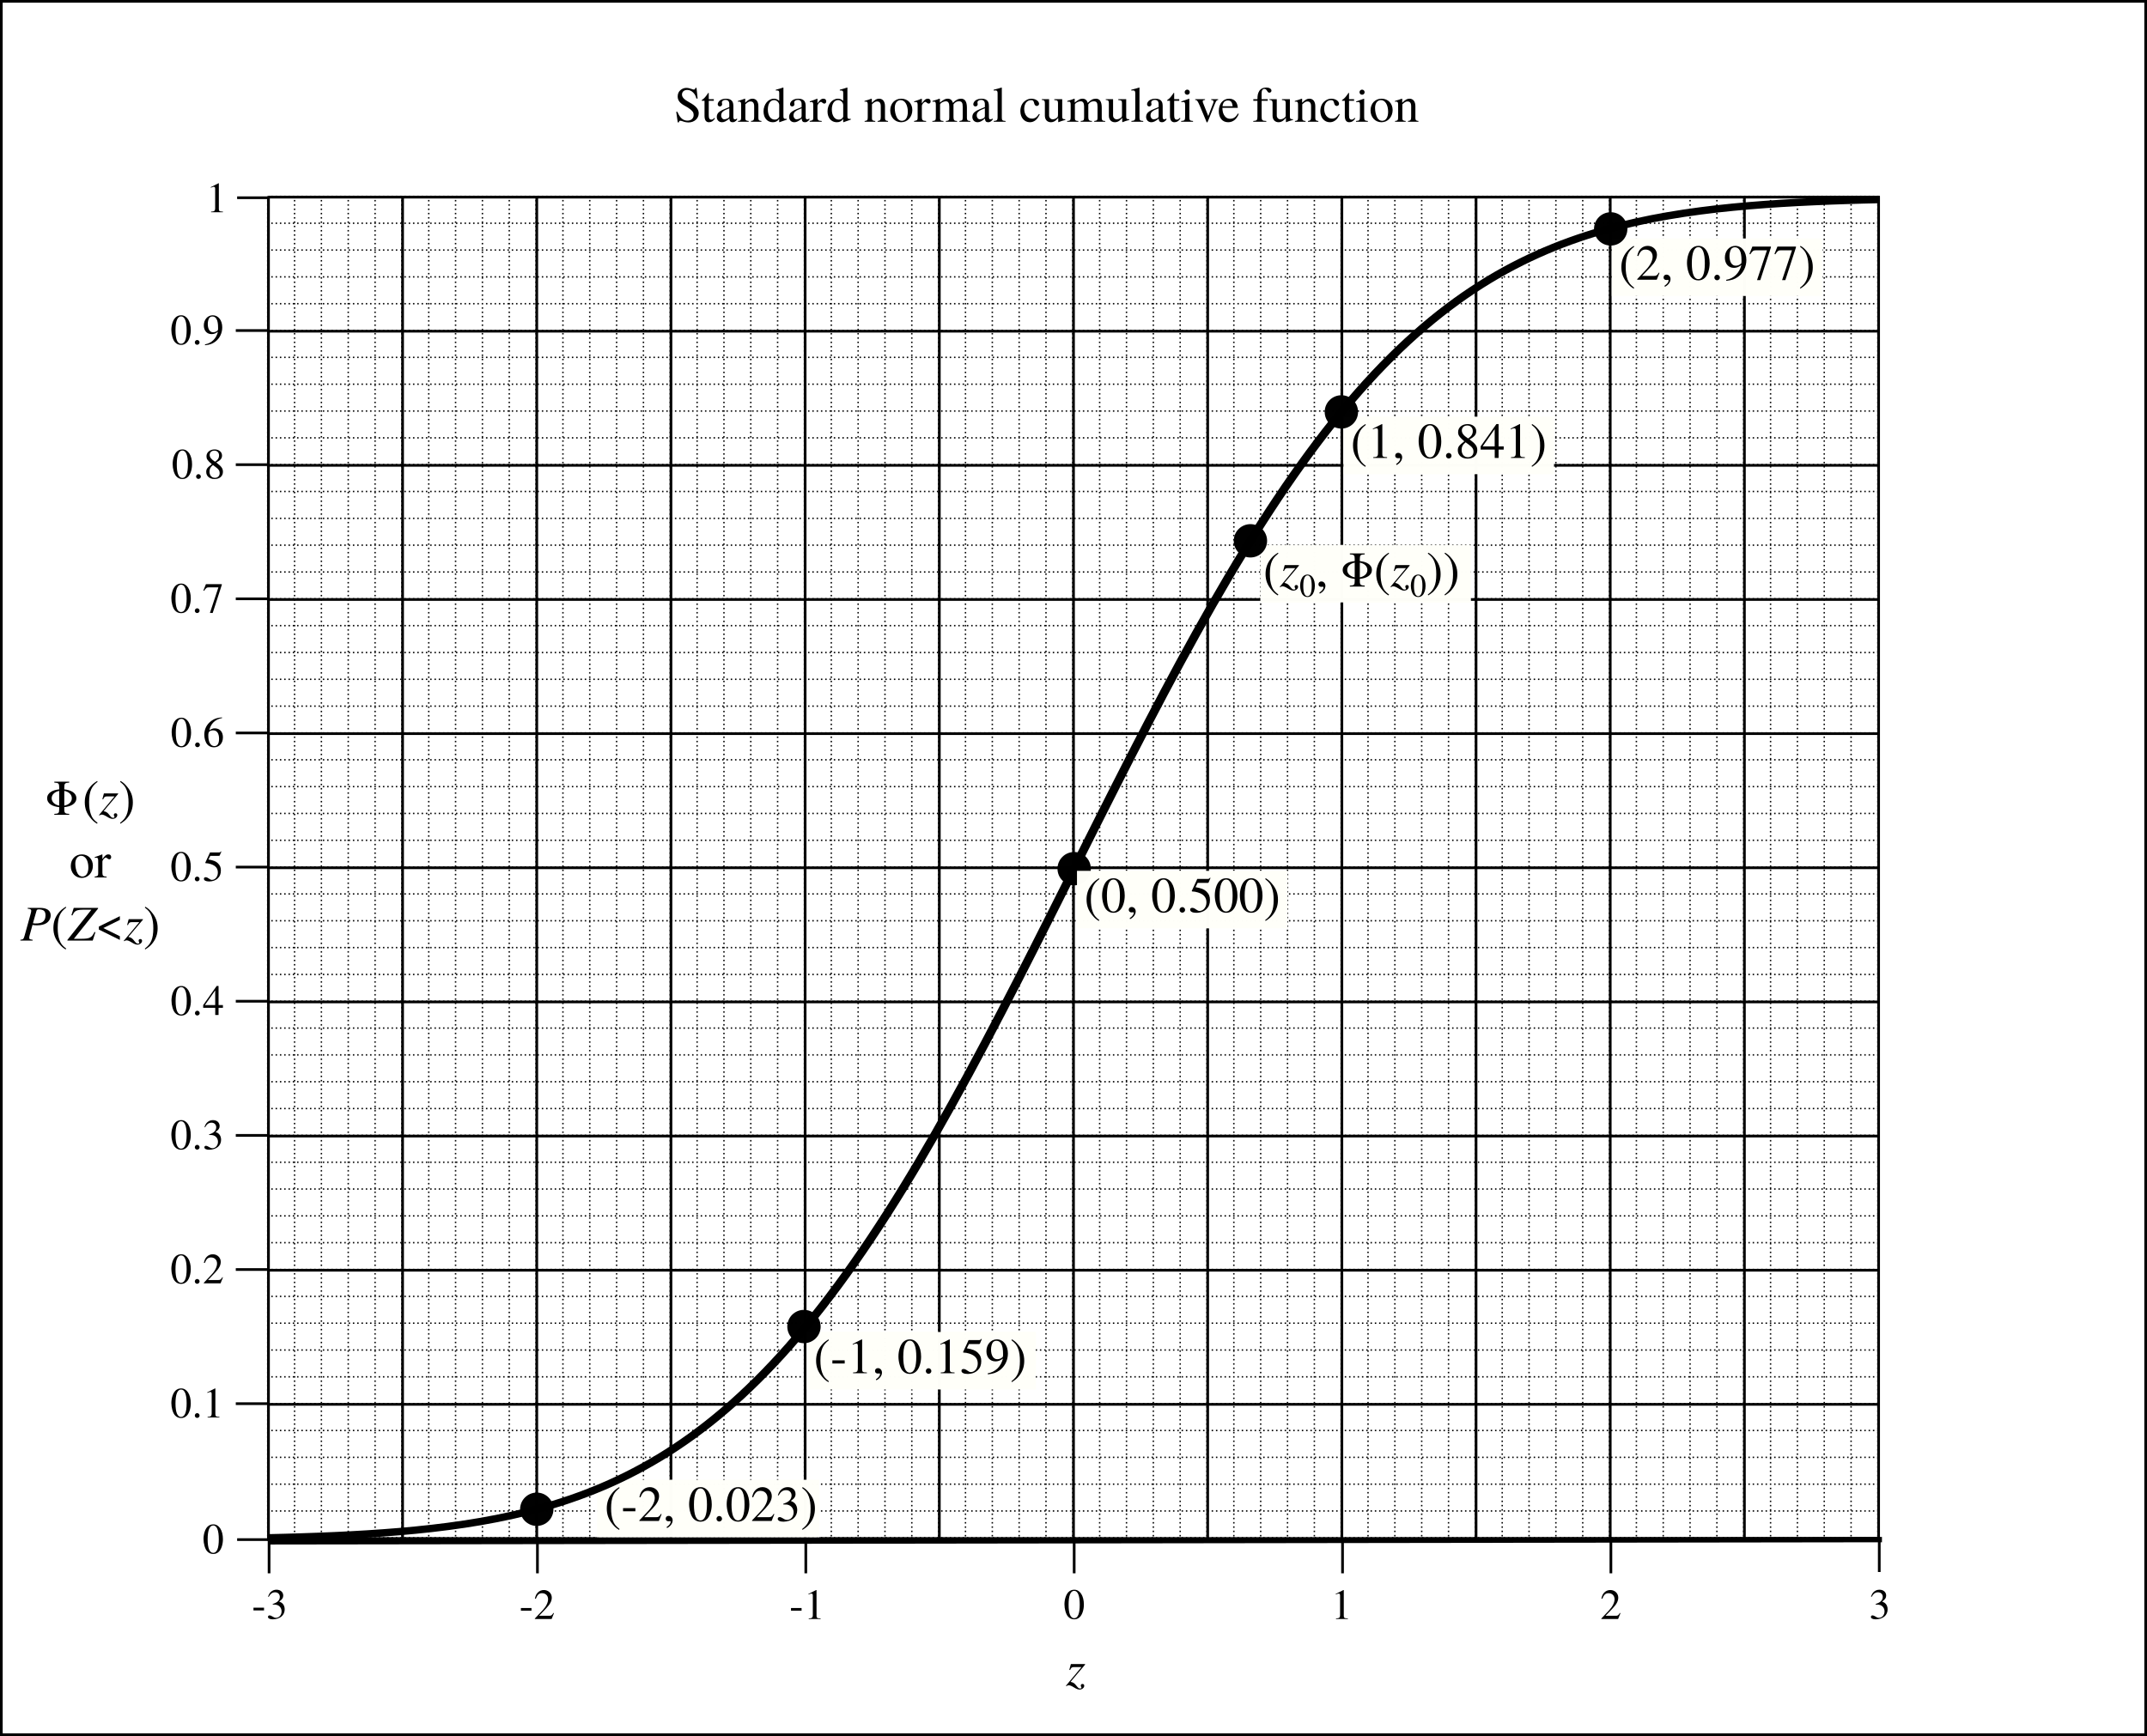
\includegraphics[scale=.65]{sncd2.png}
\end{center}
The standard normal table gives precise values of $\Phi$ as a function of $z$. (See next pages.)

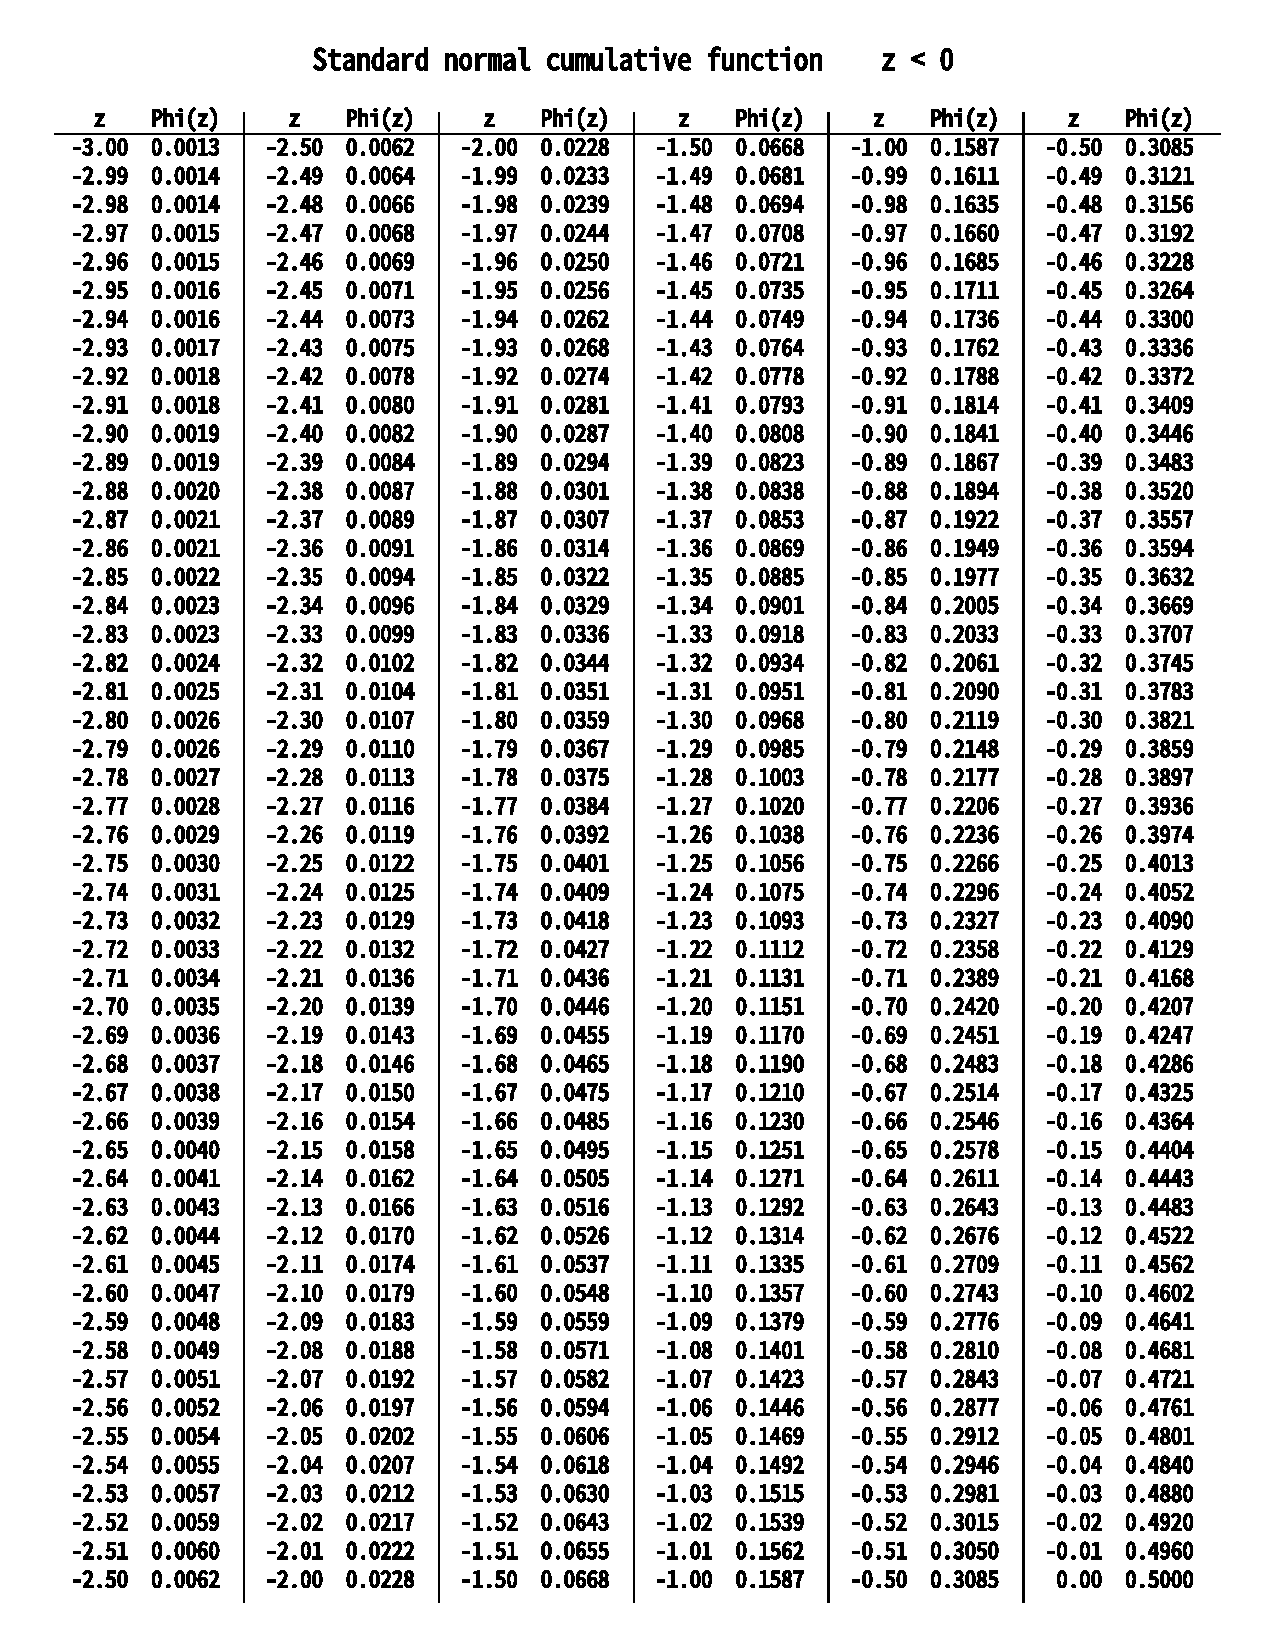
\includepdf[width=8.5in]{cumulative_neg.pdf}
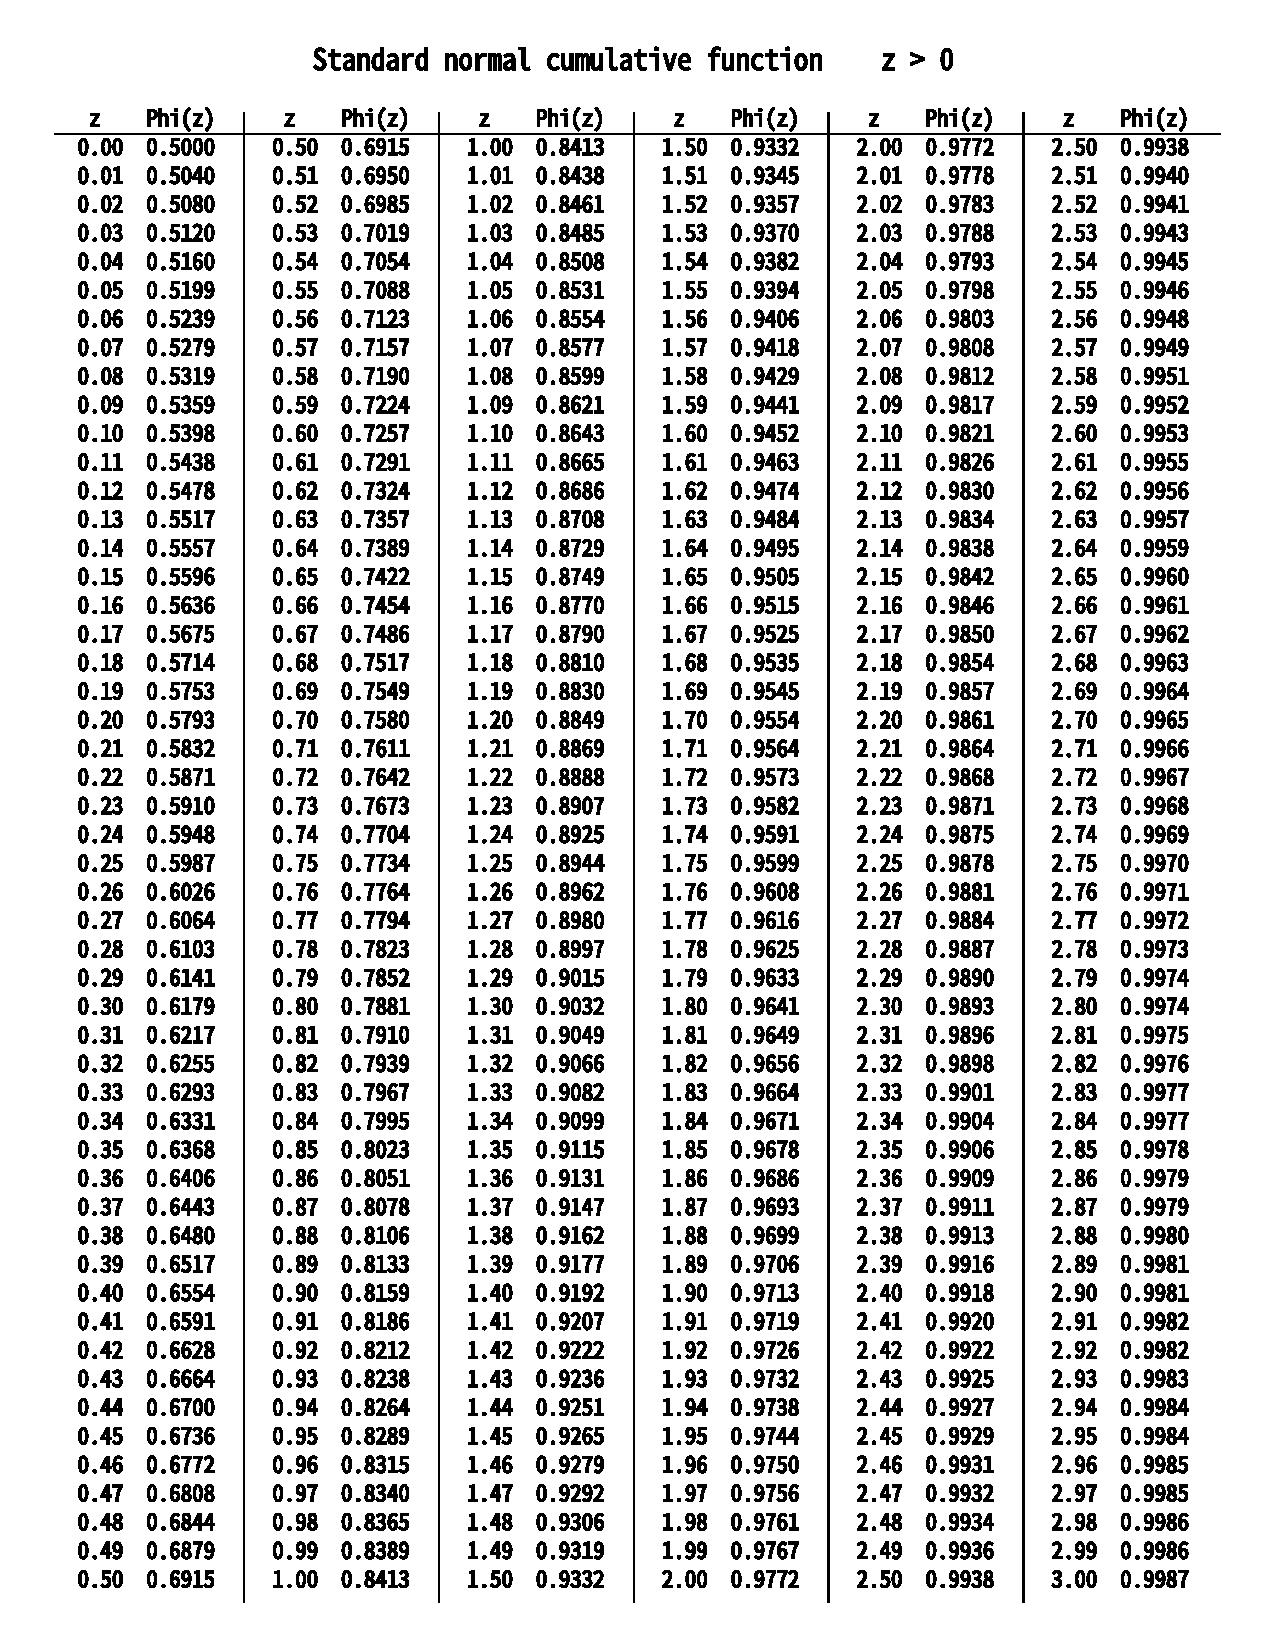
\includepdf[width=8.5in]{cumulative_pos.pdf}

Here are some useful rules. But, really, you should come up with these by sketching areas under curves. 
\begin{align*}
\textbf{Left area up to } z_0: \\
P(Z < z_0) &= \Phi(z_0) \\ \\
\textbf{Right area from } z_1: \\
P(Z > z_1) &= 1 - \Phi(z_1) \\
	       &= \Phi(-z_1)\\ \\
\textbf{Sector from } z_2 \textbf{ to } z_3: \\
P(z_2 < Z < z_3) &= \Phi(z_3) - \Phi(z_2)\\ \\
\textbf{Central area from } -z_4 \textbf{ to } z_4: \\
P(|Z| < z_4) &= \Phi(z_4) - \Phi(-z_4)\\
             &= 1-2\Phi(-z_4)\\ \\
\textbf{Two-tail area below } -z_5 \textbf{ and above } z_5: \\
P(|Z| > z_5) &= 2\Phi(-z_5)
\end{align*}

\vfill
Let $X \sim \N{\mu}{\sigma}$ and let $x$ be a specific value of $X$. You may want to convert the $x$ value into a $z$ score.
$$z ~=~ \frac{x-\mu}{\sigma}$$
You also might want to convert a $z$ score into an $x$ value.
$$x ~=~ z\sigma+\mu$$

\noindent You also might want to find $\mu$ or $\sigma$ when you know the other quantities.
$$\mu ~=~ x-z\sigma$$

$$\sigma ~=~ \frac{x-\mu}{z}$$
Notice all four of these equations represent the same relationship; we've just algebraically solved for different variables.
\vfill
%We can write rules in terms of $x$. The sector is the most general area...
%\begin{align*}
%P(x_0 < X < x_1) ~~~&=~~~ P\left(\frac{x_0-\mu}{\sigma} < Z < \frac{x_1-\mu}{\sigma}\right) \\\\
%&=~~~ \Phi\left(\frac{x_1-\mu}{\sigma}\right)-\Phi\left(\frac{x_0-\mu}{\sigma}\right)
%\end{align*}
%\vfill
\end{document}
